\subsection{Crash Course}
\begin{frame}
    \frametitle{The Very Basics}
    \begin{itemize}
        \item We look at \alert{Intel} (vs. AT\&T) style assembler
            \pedbullet{ex: MOV destination, source}
        \item Brackets are like a pointer dereference
            \pedbullet{ex: *EAX = [EAX] = dword ptr [EAX]}
        \item LEA is \alert{L}oad \alert{E}ffective \alert{A}ddress
        \begin{itemize}
            \item Transfers offset address of source to destination register
            \item It's actually faster to use the MOV instruction
                \pedbullet{ex: LEA EAX, [EBX] vs. MOV EAX, EBX}
            \item You'll see LEA frequently used for basic math operations
                \pedbullet{ex: LEA EAX, [EAX*EAX] is equivalent to $EAX^2$}
        \end{itemize}
    \end{itemize}
\end{frame}

\begin{frame}
    \frametitle{The Very Basics Continued}
    \begin{itemize}
        \item XOR-ing a register with itself zeroes it
            \pedbullet{ex: XOR EAX, EAX $\rightarrow$ EAX = 0}
        \item Numbers, signed vs. unsigned
        \begin{itemize}
            \item Unsigned positives range from \alert{0} through \alert{0xFFFFFFFF}
            \item Signed representation splits the range in half
                \pedbullet{Positives range from \alert{0x00000000} through \alert{0x7FFFFFFF}}
                \pedbullet{Negatives range from \alert{0x80000000} through \alert{0xFFFFFFFF} (-1)}
        \end{itemize}
    \end{itemize}
\end{frame}

\begin{frame}
    \frametitle{Even More Basics}
    \begin{itemize}
        \item PUSHA(D) / POPA(D)
            \pedbullet{Save / restore all registers}
        \item PUSHF(D) / POPF(D)
            \pedbullet{Save / restore all CPU flags}
        \item The 'D' instructions are 32bit, otherwise 16bit
    \end{itemize}
\end{frame}

\begin{frame}
    \frametitle{Memory Addressing Modes}
    \begin{itemize}
        \item Immediate addressing mode
            \pedbullet{\texttt{int big\_num = 0xDEADBEEF;}}
            \pedbullet{\texttt{MOV EAX, \alert{0xDEADBEEF}}}
        \item Direct addressing mode
            \pedbullet{\texttt{int big\_num = 0xDEADBEEF; b;}}
            \pedbullet{\texttt{b = *( \&big\_num );}}
            \pedbullet{\texttt{MOV EAX, \alert{[0x40508c]}}}
        \item Indirect addressing mode
            \pedbullet{\texttt{char first\_initial = *name;}}
            \pedbullet{\texttt{MOV AL, \alert{[EBX]}}}
        \item Indexed addressing mode
            \pedbullet{\texttt{int chosen = char\_array[0xC01a];}}
            \pedbullet{\texttt{MOV EAX, \alert{[EBX+0xC01A]}}}
        \item Scaled indexed addressing mode
            \pedbullet{\texttt{some\_struct *mystruct = struct\_array[20];}}
            \pedbullet{\texttt{MOV EAX, \alert{[EBX+ECX*20]}}}
    \end{itemize}
\end{frame}

\begin{frame}
    \frametitle{Instructions You Need to Know About}
    \begin{itemize}
        \item INC, DEC, ADD, SUB, MUL, DIV
            \pedbullet{Basic math instructions}
        \item MOV, LEA
            \pedbullet{Manipulate memory and registers}
        \item CALL / RET, ENTER / LEAVE
            \pedbullet{Transfer control to / back from another function}
        \item CMP, TEST
            \pedbullet{Compare values}
        \item JMP, JZ, JNZ, JG, JL, JGE, etc...
            \pedbullet{Transfer control flow to another instruction}
        \item PUSH, POP
            \pedbullet{Put items on / take items off of the stack}
        \item AND, OR, XOR, SHL, SHR
            \pedbullet{Bitwise operations}
    \end{itemize}
\end{frame}

\begin{frame}
    \frametitle{CPU Flags You Need to Know About}
    \begin{itemize}
        \item CPU flags stored in a 32-bit EFLAGS register
        \item \alert{ZF}, Zero Flag
            \pedbullet{Updated when the result of an operation is zero}
            \pedbullet{Used for JZ, JNZ etc..}
        \item \alert{SF}, Sign Flag
            \pedbullet{1 denotes negative number}
            \pedbullet{0 denotes positive number}
        \item \alert{OF}, Overflow Flag
            \pedbullet{Used in combination with ZF/SF for JG, JGE etc ...}
        \item \alert{CF}, Carry Flag (also an overflow indicator)
            \pedbullet{Used in combination with ZF for JA, JAE etc ...}
    \end{itemize}
\end{frame}


\subsection{Assembly Patterns}
\begin{frame}
    \frametitle{Calling Conventions}
    \begin{itemize}
        \item cdecl
            \pedbullet{Caller cleans up the stack}
        \item stdcall
            \pedbullet{Callee cleans up the stack}
        \item fastcall
            \pedbullet{Arguments can be passed in registers}
            \pedbullet{Microsoft: ECX and EDX (stdcall stack handling)}
            \pedbullet{Borland: EAX, ECX and EDX (also stdcall)}
        \item thiscall
            \pedbullet{C++ code, object pointer is passed in a register}
            \pedbullet{Microsoft: ECX}
            \pedbullet{Borland / Watcom: EAX}
        \item naked
    \end{itemize}
\end{frame}

\begin{frame}[fragile]
    \frametitle{Function Calls}
    \begin{columns}[T]
        \column{.5\textwidth}
            \begin{block}{stdcall}
                \begin{tiny}
                \begin{semiverbatim}
                    \alert{some_function(arg1, arg2);}

                    push arg2
                    push arg1
                    call some_function
                    mov [ebp-0xc], eax

                \end{semiverbatim}
                \end{tiny}
            \end{block}
        \column{.5\textwidth}
            \begin{block}{cdecl}
                \begin{tiny}
                \begin{semiverbatim}
                    \alert{some_function(arg1, arg2);}

                    push arg2
                    push arg1
                    call some_function
                    add esp, 8
                    mov [ebp-0xc], eax
                \end{semiverbatim}
                \end{tiny}
            \end{block}
    \end{columns}
    \begin{itemize}
        \item Function arguments are pushed in inverse order
        \item The above-left snippet demonstrates \alert{stdcall} calling convention.
            \pedbullet{The \emph{callee} cleans up the stack}
            \pedbullet{Recall that with \alert{cdecl} the \emph{caller} cleans up the stack}
        \item Can anyone guess why there is a need for stdcall vs cdecl?
    \end{itemize}
\end{frame}

\begin{frame}[fragile]
    \frametitle{EBP-Based Framing}
    \begin{columns}[T]
        \column{.5\textwidth}
            \begin{block}{Traditional}
            \begin{tiny}
            \begin{semiverbatim}
                push ebp
                mov ebp, esp
                sub esp, 0x100
            \end{semiverbatim}
            \end{tiny}
            \end{block}
        \column{.5\textwidth}
            \begin{block}{Recent OS DLLs}
            \begin{tiny}
            \begin{semiverbatim}
                mov edi, edi
                push ebp
                mov ebp, esp
            \end{semiverbatim}
            \end{tiny}
            \end{block}
    \end{columns}
    \begin{itemize}
        \item Optimized compiles may omit the frame pointer
            \pedbullet{In which case, local variables are referenced from ESP}
        \item \texttt{mov edi, edi}
            \pedbullet{Effectively a 2-byte NOP}
            \pedbullet{Why didn't they just use NOP, NOP?}
    \end{itemize}
\end{frame}

\begin{frame}
    \frametitle{Return Values}
    \begin{itemize}
        \item Saving the return value from a call
    \end{itemize}
    \begin{center}
        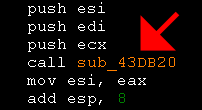
\includegraphics[scale=.75]{images/disassembly/return_value.png} \\
    \end{center}
\end{frame}

\begin{frame}[label=current]
    \frametitle{'\alert{P}' - \alert{P}arameters are \alert{P}ositive}
    \begin{itemize}
        \item \alert{P}arameters passed to a function are referenced \alert{P}ositive from EBP
            \pedbullet{\texttt{[EBP $+$ values]} are typically arguments on the stack}
            \pedbullet{\texttt{[EBP - values]} are typically local variables}
    \end{itemize}
\end{frame}

\begin{frame}[fragile]
    \frametitle{Branching}
    \begin{center}
        When reading a CMP statement, remember that the left side operand is the one being compared against.  The trick is to think \alert{"is..."}:
    \end{center}
    \begin{block}{}
        \begin{tiny}
        \begin{semiverbatim}
            ebx       = 0
            [eax+14h] = 1

            cmp     ebx, [eax+14h]  // think: \alert{is ebx...}
            ja      T1              // above? , 0 > 1 no jump
            jb      T2              // below? , 0 < 1 jumps
            je      T1              // equal? , 0 = 0 no jump
            cmp    [eax+14h], ebx   // think: \alert{is [eax+14h]...}
            ja      T2              // above? , 1 > 0 jumps
            jb      T1              // below? , 1 < 0 no jump
            je      T2              // equal? , 1 = 0 no jump
        \end{semiverbatim}
        \end{tiny}
    \end{block}
\end{frame}

\begin{frame}[fragile]
    \frametitle{Conditional Blocks}
    \begin{block}{}
        \begin{tiny}
        \begin{semiverbatim}
            \alert{if (length > 128)}
                \alert{length = 128;}

                mov eax, [ebp+8]
                cmp eax, 0x80
                jbe skip
                mov eax, 0x80
            skip:
                ...
        \end{semiverbatim}
        \end{tiny}
    \end{block}
    \begin{itemize}
        \item JBE (\alert{J}ump \alert{B}elow or \alert{E}qual) is an unsigned comparison
        \item vs. JLE (\alert{J}ump if \alert{L}ess than or \alert{E}qual) is a signed comparison
        \item While we're on the subject of signedness
            \pedbullet{MOVSX vs. MOVZX}
    \end{itemize}
\end{frame}

\begin{frame}[fragile]
    \frametitle{Loops}
    \begin{block}{}
        \begin{tiny}
        \begin{semiverbatim}
            \alert{for (i = 0; i < 100; i++)}
                \alert{do_something();}

                xor ecx, ecx
            start:
                cmp ecx, 0x64
                jge exit
                call do_something
                inc ecx
                jmp start
            exit:
        \end{semiverbatim}
        \end{tiny}
    \end{block}
    \begin{itemize}
        \item Loops are easier to spot in graphs
            \pedbullet{We'll talk more about this later}
            \pedbullet{IDA Plug-ins exist for automating loop detection}
    \end{itemize}
\end{frame}

\begin{frame}[fragile]
    \frametitle{Switch Statements}
    \begin{block}{}
        \begin{tiny}
        \begin{semiverbatim}
            \alert{switch (var) \{}
                \alert{case 0: var = 100; break;}
                \alert{case 1: var = 200; break;}
                \alert{...}

                jmp switch_table[eax*4]
            case_0:
                mov [ebp-4], 100
                jmp end
            case_1:
                mov [ebp-4], 200
                jmp end
                ...
            end:
        \end{semiverbatim}
        \end{tiny}
    \end{block}
    \begin{itemize}
        \item Both IDA and OllyDbg have excellent switch/case detection
    \end{itemize}
\end{frame}

\begin{frame}[fragile]
    \frametitle{Inline memcpy() / strcpy()}
    \begin{block}{}
        \begin{tiny}
        \begin{semiverbatim}
            mov esi, source
            mov edi, [ebp-64]
            mov ebx, ecx
            shr ecx, 2
            \alert{rep movsd}
            mov ecx, ebx
            and ecx, 3
            \alert{rep movsb}
        \end{semiverbatim}
        \end{tiny}
    \end{block}
    \begin{itemize}
        \item The \alert{rep movsd} copies ECX dwords from ESI to EDI
        \item The \alert{rep movsb} copies the remainder of the bytes
    \end{itemize}
\end{frame}

\begin{frame}[fragile]
    \frametitle{Inline strlen()}
    \begin{block}{}
        \begin{tiny}
        \begin{semiverbatim}
            mov edi, string
            or ecx, 0xFFFFFFFF
            xor eax, eax
            \alert{repne scasb}
            \alert{not ecx}
            \alert{dec ecx}
        \end{semiverbatim}
        \end{tiny}
    \end{block}
    \begin{itemize}
        \item The \alert{repne scasb} The repne scasb instruction scans the string in EDI for the character stored in AL (NULL in this case)
        \item For each scanned character ECX is decremented and EDI is incremented
        \item At the end of the REPNE sequence
            \begin{itemize}
                \item EDI = found char + 1
                \item ECX = negative string length minus two
                    \pedbullet{Logical not, minus one = string length}
            \end{itemize}
    \end{itemize}
\end{frame}

\begin{frame}[fragile]
    \frametitle{Structure Access}
    \begin{block}{}
        \begin{tiny}
        \begin{semiverbatim}
            push ebp
            mov ebp, esp
            mov \alert{eax}, off_deadbeef
            push ebx
            mov ebx, [ebp+arg_0]
            push esi
            cmp ebx, [\alert{eax}+14h]
            push edi
            ja short loc_12345678
            cmp [\alert{eax}+8], ebx
            sbb esi, esi
        \end{semiverbatim}
        \end{tiny}
    \end{block}
    \begin{itemize}
        \item EAX is loaded from a global variable
        \item Also, [] is used with EAX, which means this global variable is a pointer
    \end{itemize}
\end{frame}

\begin{frame}[fragile]
    \frametitle{Division}
    \begin{itemize}
        \item The 'div' instruction is \textbf{incredibly} slow. Compilers don't use it, unless they need the remainder
        \item Instead, divides are typically seen as a combination of shift instructions
        \item The following instruction divides EAX by 4:
            \pedbullet{\texttt{SHR EAX, 2}}
    \end{itemize}
\end{frame}

\begin{frame}[fragile]
    \frametitle{Pseudo Random Numbers}
    \begin{block}{Slammer MSSQL Worm PRND Engine}
        \begin{tiny}
        \begin{semiverbatim}
            MOV    0XFFFFFFB4(%EBP),%EAX ; eax = GetTickCount()
            LEA    (%EAX,%EAX,2),%ECX    ; ecx = eax + eax * 2
            LEA    (%EAX,%ECX,4),%EDX    ; edx = eax + ecx * 4
            SHL    $0X4,%EDX             ; edx = edx << 4 (edx *= 2^4 (16))
            ADD    %EAX,%EDX             ; edx += eax
            SHL    $0X8,%EDX             ; edx = edx << 8 (edx *= 2^8 (256))
            SUB    %EAX,%EDX             ; edx -= eax
            LEA    (%EAX,%EDX,4),%EAX    ; eax = eax + edx * 4
            ADD    %EBX,%EAX             ; eax += ebx
            MOV    %EAX,0XFFFFFFB4(%EBP) ; store target address
        \end{semiverbatim}
        \end{tiny}
    \end{block}
    \begin{itemize}
        \item Sorry, this is a different flavor of assembly (old excerpt)
        \item "Random" numbers are frequently generated via large multiplications that rely on integer wrapping
        \item The above excerpt is equivalent to multiplying by 214,013
    \end{itemize}
\end{frame}

\begin{frame}
    \frametitle{Type Recovery}
    \begin{itemize}
        \item There is no type representation at the assembly level
        \item We need to differentiate...
            \pedbullet{Strings from raw data}
            \pedbullet{UNICODE strings from ASCII strings}
            \pedbullet{Integers from pointers}
            \pedbullet{Integers from booleans}
        \item Sometimes type recovery requires examination across function boundaries
        \item Type recovery is simple for documented API calls
    \end{itemize}
\end{frame}

\begin{frame}
    \frametitle{Type Recovery: Integers vs. Pointers}
    \begin{itemize}
        \item Integers are \alert{never} dereferenced
        \item Integers are frequently compared, pointers are not
        \item Pointers are compared against zero or other pointers
        \item Arithmetic on pointers is simple, potentially complex for integers
    \end{itemize}
\end{frame}

\begin{frame}
    \frametitle{Type Recovery: Strings vs. Raw Data}
    \begin{itemize}
        \item String copying is generally prefixed with a strlen() (or inline equivalent)
            \pedbullet{Raw data copies will not have a prefixed strlen()}
        \item Strings are often compared against readable characters and other strings
            \pedbullet{Raw data may not be}
        \item Trace string parameters down to API calls!
    \end{itemize}
\end{frame}

\begin{frame}[fragile]
    \frametitle{C++ (Object Oriented) Code}
    \begin{itemize}
        \item As mentioned before, the \alert{this} pointer is typically passed to function through ECX
    \end{itemize}
    \begin{block}{}
        \begin{tiny}
        \begin{semiverbatim}
            lea ecx, [esp+16]
            call member_routine
        \end{semiverbatim}
        \end{tiny}
    \end{block}{}
    \begin{itemize}
        \item Virtual Tables or VTables, are commonly seen in C++. Example:
    \end{itemize}
    \begin{block}{}
        \begin{tiny}
        \begin{semiverbatim}
            mov eax, esi
            push 0x100
            call dword ptr [eax+50]
        \end{semiverbatim}
        \end{tiny}
    \end{block}{}
    \begin{itemize}
        \item When reversing arbitrary objects or structures locating initialization routines such as constructors / destructors can prove helpful
    \end{itemize}
\end{frame}

\begin{frame}
    \frametitle{Branchless Logic}
    \begin{itemize}
        \item Compilers will avoid branching if possible
        \item Many simple compare / branch pairs can be converted into a sequence of arithmetical operations
        \item The usage of the \alert{\texttt{sbb}} instruction is a typical indicator
        \item The resulting code runs faster, but is not as readable for human analysis
    \end{itemize}
\end{frame}

\begin{frame}[fragile]
    \frametitle{Branchless Logic: Example}
        \begin{block}{}
            \begin{semiverbatim}
                cmp     eax, 1
                sbb     eax, eax
                inc     eax
                pop     esi
                pop     ebx
                retn
            \end{semiverbatim}
        \end{block}
        \begin{itemize}
            \item<+-> \alert{cmp eax, 1} will set the carry flag (\alert{CF}) if \alert{eax} is 0
            \item<+-> \alert{sbb eax, eax} does \alert{eax = eax - (eax+CF)}
            \item<+-> Therefore if \alert{eax} was 0 we have \alert{eax = 0 - (0+1) = -1}
            \item<+-> Otherwise if \alert{eax} is greater than 0 we have \alert{eax = eax - eax+0 = 0}
            \item<+-> The increment will set the possible \alert{eax} values to 1 or 0
        \end{itemize}
\end{frame}

\begin{frame}[fragile]
    \frametitle{Mastering These Concepts}
    \begin{itemize}
        \item Reverse engineering isn't as much a matter of difficulty as it is a matter of familiarization and practice
        \item The best way to learn is hands on experience
            \begin{itemize}
                \item Keep a quick reference handy (see opcodes.hlp)
                \item Single step with a debugger
                \item Use an emulator
                \item Disassemble familiar code
                    \pedbullet{Compile and disassemble small snippets of code}
            \end{itemize}
    \end{itemize}
\end{frame}
